\chapter{Theoretical Background and Related Work}
This section outlines key findings of related work on gender bias in MT, with a focus on the English-German (EN-DE) language pair to build the theoretical knowledge base. The research aims are to (1) define the core concept of gender bias in MT, (2) establish the relevance of the topic, (3) identify the research gap, and (4) justify technical design choices. 

For the literature review I combined incremental and conceptual literature review methods, where each source led to the identification of the next. Based on this progression, I identified key concepts and used them to organize and interpret the literature, aligning with a conceptual approach. The structure followed the qualitative Information Systems framework by \citet{schryenWritingQualitativeLiterature2015} and was further informed by \citet{shresthaExploringGenderBiases2022} and \citet{savoldiDecadeGenderBias2025}, who both conducted systematic reviews on gender bias in ML and MT respectively. 

% --------------------------------------------------------------------------------
\section{Literature Search Process}

\subsection{Search Sources and Tools}
Sources were primarily searched on \href{https://scholar.google.com/}{Google Scholar} and \href{https://www.perplexity.ai/}{Perplexity}, which served as an additional search engine. Prompts and outputs from Perplexity have been saved and are included in the appendix. To organize and manage the collected sources, \href{https://www.zotero.org/}{Zotero} was used throughout the process.

\subsection{Literature Review Framing}

To answer the four research aims, I have defined the key concepts in \autoref{tab:key-concepts}. Key search terms consisted of \textit{gender bias}, \textit{machine translation}, \textit{AI}, \textit{machine learning}, \textit{German}, \textit{stereotypes}, and \textit{detection}, which were combined with \textit{AND/OR}. The focus was on literature published between 2019 and 2025 to maintain relevance and currency, while foundational and definitional works from earlier periods were selectively included. The initial search for the term \textit{gender bias in machine translation} returned over 18,000 results. Through my iterative selection process, this was narrowed down to 34 core sources.

\renewcommand{\arraystretch}{1.3}
\begin{table}[ht!]
\centering
\begin{tabularx}{\textwidth}{>{\raggedright\arraybackslash}p{6.5cm}X}
\toprule
\textbf{Key Concept} & \textbf{Description} \\
\midrule

Foundations of Gender Bias in Natural Language Processing & Traces early research that identified gender bias in language. Focuses on foundational studies that showed why the issue matters and how later work builds on these findings. \\

Sources and Manifestations of Bias & Explains how stereotypes shape language and persist over time. Describes how societal bias enters training data, model design, and system feedback. Shows how bias appears in machine translation and everyday language. \\

Linguistic Challenges in English-German Translations & Explores key grammatical differences between English and German that affect translation. Focuses on how the lack of gender in English and its presence in German can lead to biased outputs. \\

Mitigation Strategies and Current Limitations & Reviews how current research tries to reduce gender bias in NLP. Highlights what these methods can and cannot do. Helps identify where a classification-based approach could fill gaps and improve bias detection in translations. \\

\bottomrule
\end{tabularx}
\caption{Key concepts relevant to this thesis}
\label{tab:key-concepts}
\end{table}


\subsection{Citation Tracking}
Backward citation searching involved reviewing references cited by selected papers, prioritizing frequently cited and foundational works relevant to gender bias in MT. Forward citation searching used Google Scholar's "cited by" function to identify newer research citing those key papers. Filtering with specific terms (e.g., \textit{German} and \textit{machine translation}) was applied during forward search to maintain focus. Beyond these systematic methods, I also included supplementary sources when needed while writing. These consist of contextual references, statistics, or secondary citations that support specific points but were not part of the core conceptual or methodological framework. Supplementary sources were defined as materials identified outside the systematic search, such as papers found through backward citations or targeted queries for statistics and news, which provided support for subordinate arguments without being central to the study's theoretical or analytical structure.



\subsection{Selection Criteria and Screening Process}\label{subsection:selection_criteria}
Titles and abstracts were manually screened to select relevant studies. \textbf{Inclusion criteria} required sources to specifically address gender bias in MT, provide examples or discussions of gender-related errors, or explain the significance of gender bias in this context. Sources also had to be available in full text without access restrictions. \textbf{Exclusion criteria} filtered out studies focusing on general NLP bias without a direct link to MT, non-gender biases, and highly technical papers lacking contribution to the general understanding of gender bias or that did not provide additional knowledge beyond what was already found in previously published papers. Full texts were reviewed after initial screening to confirm relevance and extract insights. Redundant sources not providing new perspectives aligned with the thesis goals were excluded.

% --------------------------------------------------------------------------------

\section{Understanding Gender Bias in English-to-German Machine Translation}

This section explains the key terms and concepts needed to understand gender bias in English-to-German MT. It defines important ideas like natural language processing (NLP), MT, and gender bias. These concepts provide the background necessary to follow the thesis.

\subsection{Differentiating between Natural Language Processing and Machine Translation}
\textbf{NLP} refers to the development of machine systems that can process and generate human language. The goal is to mimic and understand it as fluently as possible \citep{smacchiaDoesAIReflect2024,ullmannGenderBiasMachine2022}. Common applications are chatbots, translation tools, speech recognition, and image captioning.

\textbf{MT} is a direct application of NLP. It is used to automatically translate text from one language to another \citep{linMachineTranslationAcademic2009}. MT systems have gone through several stages of development; earlier approaches like rule-based and statistical MT used manually defined grammar rules or pattern matching from large translation corpora \citep{chakravarthiSurveyOrthographicInformation2021}. For example:

\begin{quote}
"The girl reads a book" → "Das Mädchen liest ein Buch"\\[0.5em]
Rules: "girl" → "Mädchen", "reads" → "lesen", "book" → "Buch"
\end{quote}

\noindent These systems often struggled with full sentences and complex expressions because they fail to capture context and phrase-level meaning. "She gave him a hand" might be translated literally, missing its idiomatic meaning.

Most modern systems, including Google Translate and DeepL, use \textbf{neural machine translation (NMT)} \citep{wuGooglesNeuralMachine2016,deeplHowDoesDeepL2021}. These systems are trained on large sets of translated texts. They learn to represent the meaning of whole sentences as mathematical structures and generate more fluent and accurate translations. Unlike earlier systems, they aim to consider the full context of a sentence, which helps reduce errors and improves the handling of ambiguous or idiomatic language.

\subsection{How Bias Enters Machine Translation Systems}

Similarly to how humans are shaped by their environemnt, MT models learn from data they are trained on. Existing biases are thus reflected and reinforced in the final models, creating "machine bias" \citep{stanczakSurveyGenderBias2021,smacchiaDoesAIReflect2024}. \citet{shahPredictiveBiasesNatural2020}, as described by \citet{ullmannGenderBiasMachine2022}, differentiates between four origins of biases affecting NLP systems:

\begin{itemize}
    \item \textbf{Selection Bias:} Happens when the training data does not reflect the context in which the model is used (e.g., using Wikipedia data for detecting harmful language on Twitter).
    
    \item \textbf{Label Bias:} Occurs when annotations in the dataset are incorrect or skewed. This can be influenced by the annotators' own biases or lack of awareness of diverse linguistic expressions.

    \item \textbf{Model Overamplification:} During training, models can exaggerate patterns found in the data. If a dataset predominantly associates cooking with women, the assumption can be reinforced that cooking is an activity exclusive to women.

    \item \textbf{Semantic Bias:} Stems from associative relationships within the data, where certain words or phrases are frequently co-occurring with specific genders (e.g., "he" with "doctor").
\end{itemize}

\citet{ullmannGenderBiasMachine2022} notes that the scale of training data (e.g., 175 billion parametres for GPT-3) makes it practically impossible to review all of it, allowing misinformation or offensive content to be reproduced by the system. The author also points out that platforms like Wikipedia and Reddit are male-dominated and often contain harmful or false content.

\subsection{What Gender Bias Means in Machine Translation}

A clear definition of gender bias has not yet been established \citep{stanczakSurveyGenderBias2021}. Determining which features in text indicate bias is difficult, and the characteristics of non-biased text are often unclear. This makes it challenging to hold users accountable for gender bias, detect all harmful signals, and develop standard evaluation benchmarks \citep{barclayInvestigatingMarkersDrivers2024a,shresthaExploringGenderBiases2022,stanczakSurveyGenderBias2021}. 

Since there is no clear definition, this work defines gender bias based on specific manifestations described in the following subsection. Any text that exhibits one or more of these forms will be considered gender biased.

\subsection{Manifestiations of Gender Bias}
This section draws from the main studies analyzing gender bias in EN-DE MT \citep{ullmannGenderBiasMachine2022,rescignoGenderBiasMachine2023,lardelliBuildingBridgesDataset2024,kapplAreAllSpanish2025}. Since existing research does not clearly define the different manifestations, the findings are grouped here into three main categories.

\subsubsection{Defaulting to Masculine Forms}
In both singular and plural contexts, the \textit{generic masculine} refers to the default use of the masculine grammatical gender.
For example, the sentence "Die Studenten sind im Hörsaal" (translation: "The students are in the lecture hall") uses the masculine plural form to refer to a group of students regardless of their gender.

It is commonly used in spoken German \citep{lardelliBuildingBridgesDataset2024,schmitzGermanAllProfessors2022}, although research has consistently shown that the generic masculine creates a male bias in mental representations, leading readers or listeners to think more of male than female examples \citep{sczesnyCanGenderFairLanguage2016}. In MT, the generic masculine can lead to inaccurate or unfair representations of gender in translated text. \citet{rescignoGenderBiasMachine2023} observed a predominance of masculine forms in translation outputs (approximately 90\% in Google Translate and 85–88\% in DeepL for EN-IT and EN-DE), even when the original sentences contained relatively few masculine references. This shows that the bias is not minor but occurs quite heavily in those systems.


\subsubsection{Reinforcement of Stereotypes}
Stereotypes and gender roles stem from historical and cultural perceptions of men's and women's societal roles, many of which are obsolete but still influential. For example, when men and women often take on different roles at work and at home, it shapes how people think about their personalities and qualities. Correspondence bias can emerge, where people infer attributes from observable behaviours \citep{godsilEffectsGenderRoles2016}. These associations can then be reinforced by popular media, such as TV and advertisements \citep{godsilEffectsGenderRoles2016}, just as much as it can be influenced by MT tools.

A common manifestation of this are \textbf{stereotypical job associations}. This can be seen in cases where models assign he/him pronouns to roles like doctors and pilots, and she/her pronouns to roles like nurses and flight attendants \citep{shresthaExploringGenderBiases2022}, with an even stronger tendency in male-domniated fields such as STEM \citep{pratesAssessingGenderBias2019}. In addition, NLP models have also been shown to \textbf{link certain adjectives and traits to genders}. Traits like "masterful," "assertive," and "competitive" are often associated with men, while "friendly," "unselfish," and "emotionally expressive" are more commonly linked to women \citep{godsilEffectsGenderRoles2016}.

\subsubsection{Neglecting Contextual Information}

\textbf{Coreference resolution} refers to the process of using contextual information to determine the correct gender in translation \citep{stanczakSurveyGenderBias2021}. In MT, this means identifying links between words like pronouns and the nouns they refer to. While human translators use both linguistic cues (such as pronouns and grammar) and real-world knowledge to correctly assign gender \citep{rescignoGenderBiasMachine2023}, MT systems often fail to do so reliably, especially when gender information appears earlier in the text or across sentence boundaries \citep{choMeasuringGenderBias2019,stanovskyEvaluatingGenderBias2019}. For example, if a biography introduces a person with a female name at the beginning, but later refers to that person only by name, translation systems may lose the link and default to masculine forms for the remaining text.

\citet{rescignoGenderBiasMachine2023} found that including previous sentences improved coreference resolution and reduced masculine defaults, though some systems benefited more than others. However, the use of context also introduced occasional new errors. Additionally, \citet{savoldiWhatHarmQuantifying2024} highlighted that correcting biased translations toward feminine forms required significantly more time and edits than masculine ones, revealing a notable cost disparity.

Similarly, \citet{lardelliBuildingBridgesDataset2024} showed that even with natural passages from Wikipedia and Europarl, systems still largely defaulted to masculine forms. Feminine and inclusive translations remained rare, while gender-neutral alternatives appeared mainly when the noun itself suggested them.


\subsection{Linguistic Challenges in English-German Translation}

Although both English and German originate from the Indo-European language family \citep{baldiEnglishIndoEuropeanLanguage2008}, they have different characteristcs. English does not assign grammatical gender to nouns. The article "the" is used universally, independent of what it refers to. On the contrary, German assigns one of three grammatical gendered articles to nouns: "der" (m), "die" (f) and "das" (n). The form or ending of a noun may also change depending on its grammatical gender. While English has a few gendered word pairs, such as "actor" (m) and "actress" (f), gender distinctions in German apply broadly across the entire noun system. "Der Student" refers to a male student, whereas "die Studentin" refers to a female student. Note that grammatical gender has no connection to societal or biological gender. It is a rule of the language rather than a reflection of identity. For example, the German word Mädchen (girl) is grammatically neuter and takes the article "das". This is not because the referent lacks gender, but because the suffix "-chen" automatically assigns neuter gender. Grammatical gender in German follows structural rules, even when they contradict real-world gender associations.

\subsection{German Gender-Fair Language}
Gender-fair language (GFL) refers to the use of language that treats all genders equally and aims to reduce stereotyping and discrimination \citep{sczesnyCanGenderFairLanguage2016}. Three common approaches to plural mentionings in German are: 

\begin{itemize}
    \item \textbf{Gender-neutral rewording:}  
    This uses neutral terms instead of gendered nouns, e.g., \textit{die Studierenden lernen}. A challenge for this version is that neutral alternatives do not exist for every noun and cannot be consistently applied \citep{lardelliBuildingBridgesDataset2024}.

    \item \textbf{Gender-inclusive characters:}  
    This combines masculine, feminine and non-binary forms by using a character like \textit{*}, \textit{:}, or \textit{\_}, e.g., \textit{die Student*innen lernen}. This method is consistent but may interrupt reading flow and lacks standardization \citep{lardelliBuildingBridgesDataset2024}.

    \item \textbf{Pair form:}  
    This names both gender forms, e.g., \textit{die Studentinnen und Studenten lernen}. It is currently the most used GFL form in German \citep{waldendorfWordsChangeIncrease2024}, briefly surpassing the star and colon characters as seen in \autoref{fig:gfl_types_frequency}.
\end{itemize}

These examples apply when the gender of the subjects is ambiguous. But when gender is known, especially in singular mentions, the generic masculine should be avoided. However, in the same way as gender bias has no clear definition, there is \textbf{no agreed standard for GFL} \citep{lardelliBuildingBridgesDataset2024, savoldiDecadeGenderBias2025}. "Fairness" therefore heavily depends on personal views, culture, and context, which raises ethical questions about debiasing systems.

\begin{figure}
	\centering
		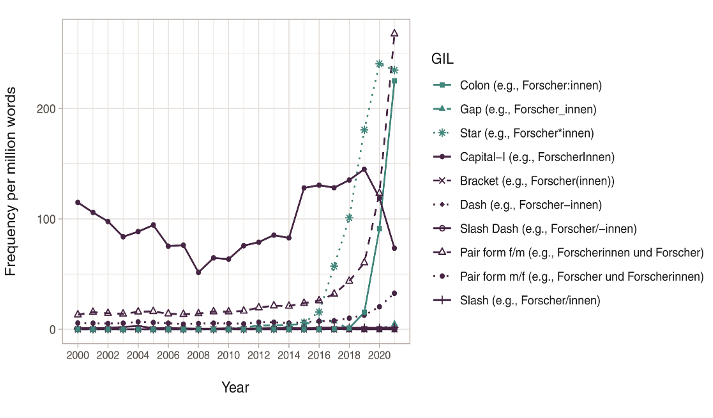
\includegraphics[width=1\textwidth]{gfl_types_frequency.png}
	\caption{Frequency of different types of gender-inclusive language. Source: \citet{waldendorfWordsChangeIncrease2024} p. 367.}
	\label{fig:gfl_types_frequency}
\end{figure}

% --------------------------------------------------------------------------------

\section{Societal Relevance and Impact of Gender Bias in Machine Translation}

This section outlines why gender bias is a subject of research in the first place and where it connects to broader social and ethical questions. It first looks at early studies that brought attention to gender patterns in language technologies and raised awareness of their social impact. Understanding these origins helps explain why it continues to be relevant today.

\subsection{Foundational studies}
The existence of gender bias in MT is well-documented. First mentions of this issue date back to over a decade ago, having been recognized by a paper by \citeauthor{schiebingerScientificResearchMust2014} in 2014. Since then, there has been a general increase in research papers focusing on this topic, especially between 2019 and 2023 \citep{savoldiDecadeGenderBias2025}.

\textbf{\citet{pratesAssessingGenderBias2019}} conducted a large-scale study using Google Translate to translate sentences like "[Gender-neutral pronoun] is an engineer" from twelve gender-neutral languages into English. The results showed a strong bias toward male pronouns, especially in STEM occupations. This could not be explained by real-world labor statistics, pointing instead to imbalances in the system's training data. The study received wide media attention, leading \citeauthor{googleReducingGenderBias2018} to change their translation policy: Google Translate began showing both feminine and masculine forms for ambiguous inputs \citep{googleReducingGenderBias2018} (see \autoref{fig:gt_prates_example}).

Building on this, \textbf{\citet{stanovskyEvaluatingGenderBias2019}} created \href{https://github.com/gabrielStanovsky/mt_gender}{WinoMT}, a benchmark for evaluating gender bias in English-to-multilingual translations. It focused on occupations in contexts designed to challenge stereotypes. The study found that systems were more accurate for stereotypical gender roles but struggled in non-stereotypical cases, confirming the trends observed by \citeauthor{pratesAssessingGenderBias2019}.
Together, these studies helped spark the ongoing research interest in gender bias in MT.

\subsection{Why it matters}
Gender bias in MT can lead to \textbf{representational harm}, meaning biased or reductive portrayals of a particular gender continue to spread \citep{stanczakSurveyGenderBias2021}.

It also contributes to the invisibility of women in male-dominated professions \citep{kapplAreAllSpanish2025}. Studies show that biased language in machine-generated text, such as children’s stories or job ads, can \textbf{influence how young people view themselves} \citep{soundararajanInvestigatingGenderBias2024,kapplAreAllSpanish2025}. It may shape their interests, hobbies, and career choices. This is especially visible in STEM fields \citep{pratesAssessingGenderBias2019}, where stereotypes are more persistent. When job descriptions or mock interviews use gender-exclusive pronouns, women report feeling less belonging, lower motivation, and weaker identification with the role \citep{godsilEffectsGenderRoles2016}. Many self-select out of applying, shrinking the female talent pool and \textbf{reinforcing gender gaps in the workforce}.

Research also shows that using GFL like "she and he" or "one" can improve how women respond to job ads. It reduces stereotype threat and helps them engage more positively with opportunities \citep{godsilEffectsGenderRoles2016}. Using inclusive language can therefore offer both social and competitive benefits for companies.

Furthermore, a study by \citet{savoldiWhatHarmQuantifying2024} employed behavioral metrics such as time to edit and the number of edits, measured through human-targeted error rate, to quantify the effort required. The results showed that post-editing feminine translations required nearly twice as much time and four times the number of editing operations compared to masculine counterparts (\autoref{fig:savoldi_post_editing}). Consequently this effort gap also translates into \textbf{higher economic costs}, suggesting a measurable \textbf{quality-of-service disadvantage that disproportionately affects women}. \citeauthor{savoldiWhatHarmQuantifying2024} concluded that current automatic bias metrics do not sufficiently capture these human-centered disparities, emphasizing the need for evaluation methods that reflect real user experience.

\begin{figure}
	\centering
		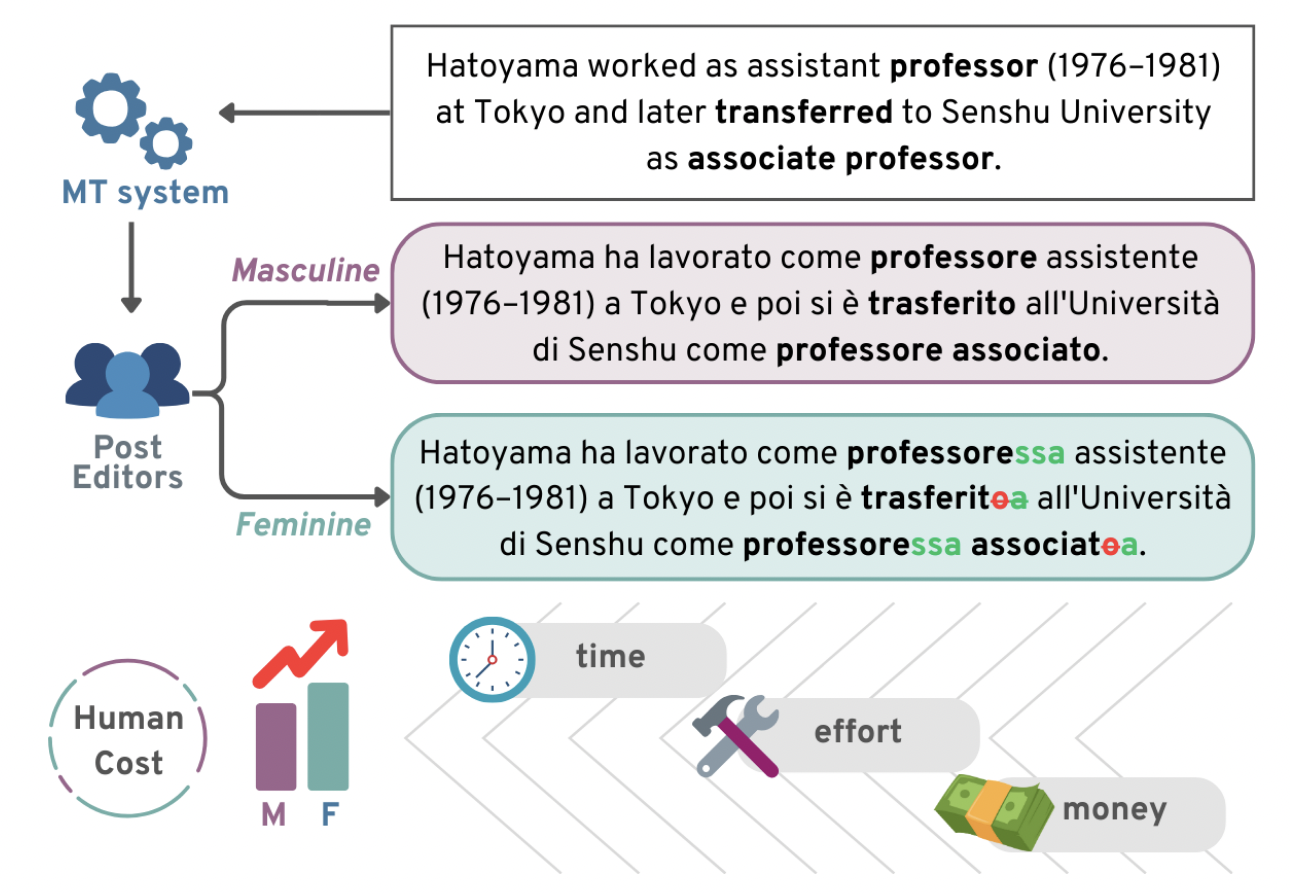
\includegraphics[width=1\textwidth]{savoldi_post_editing.png}
	\caption{Study design. Post-editing of an MT output into both feminine and masculine gender. Source: \citet{savoldiWhatHarmQuantifying2024} p. 18048}
	\label{fig:savoldi_post_editing}
\end{figure}

% --------------------------------------------------------------------------------

\section{Research Gaps}

% --------------------------------------------------------------------------------

\section{Approach and Justification of the Technical Setup}

